\pstart  At non defuere qui se Hypothesi  de Aeris gravitate\protect\index{Sachverzeichnis}{gravitas!aeris} opponerent, \edtext{quorum}{\lemma{opponerent,}\Afootnote{ \textit{ (1) }\ ex quibus \textit{ (2) }\ quorum \textit{ L}}}  Doctus Hyperaspistes, Franciscus Linus\protect\index{Namensregister}{\textso{Linus,} Franciscus 1595\textendash 1675} Funiculum\protect\index{Sachverzeichnis}{funiculus} quendam introduxit,\edtext{}{\lemma{introduxit,}\Bfootnote{\textsc{F. Linus, }\cite{00072}\textit{Tractatus de corporum inseparabilitate}, London 1661, S.~27.}} cujus hic sensus est \edtext{Mercurium}{\lemma{est}\Afootnote{ \textit{ (1) }\ aerem \textit{ (2) }\ Mercurium \textit{ L}}}, in Tubo Torricelliano\protect\index{Sachverzeichnis}{Tubus!Torricellianus}
[97 v\textsuperscript{o}] descendentem non ultra descendere, quam Materiam subtilem\protect\index{Sachverzeichnis}{materia!subtilis}, (sive aerem, sive aliud nescio quid) tendere  seu dilatare possit. Eam enim ulteriori dilatationi  reniti, ac proinde Mercurium\protect\index{Sachverzeichnis}{mercurius} amplius non descendere,  at augeri descensum \edtext{proportione Tubi}{\lemma{descensum}\Afootnote{ \textit{ (1) }\ seu suspensionem esse eandem Tubo \textit{ (2) }\  ab \textit{ (3) }\ ultra imum \textit{ (4) }\ proportione Tubi \textit{ L}}} aucti, \edtext{ seu locum Mercurii nondum delapsi infimos 30 pollices}{\lemma{aucti,}\Afootnote{ \textit{ (1) }\ semper \textit{ (2) }\ seu suspensionem ultra partem residuam \textit{ (3) }\ et \textit{ (4) }\  vel 30 pollices infimos Mercurii\protect\index{Sachverzeichnis}{mercurius|textit} suspensi semper \textit{ (5) }\ seu [...] pollices \textit{ L}}} continentem, post reliqui delapsum semper summos 30 Mercurii\protect\index{Sachverzeichnis}{mercurius} pollices retinere; quia  si altior \edtext{lapsus}{\lemma{altior}\Afootnote{ \textit{ (1) }\ Tubus \textit{ (2) }\ lapsus \textit{ L}}} ac proinde major spatii relicti tensio\protect\index{Sachverzeichnis}{tensio},  etiam \edtext{majus}{\lemma{etiam}\Afootnote{ \textit{ (1) }\ fortius \textit{ (2) }\ majus \textit{ L}}} est pondus Mercurii\protect\index{Sachverzeichnis}{mercurius} tendentis seu delabentis, quod spatium lapsus impleverat.
\pend 
\pstart  Haec sententia a multis cum plausu recepta est. Rationem  enim reddere \edtext{potest plerorumque}{\lemma{potest}\Afootnote{ \textit{ (1) }\ omnium \textit{ (2) }\ plerorumque \textit{ L}}} phaenomenorum, ut quod  in \edtext{montis vertice}{\lemma{in}\Afootnote{ \textit{ (1) }\ alto monte \textit{ (2) }\ montis vertice \textit{ L}}} minor Baroscopii\protect\index{Sachverzeichnis}{baroscopium!Torricellianum} altitudo,  quia non tantum aer intus tensus retinet, sed et  aer in alto extrorsum tensior attrahit. Unde  etiam ratio reddi posset cur in Recipiente Magdeburgico\protect\index{Sachverzeichnis}{Recipiens!Magdeburgicum} \edtext{liquor}{\lemma{}\Afootnote{liquor \textit{ erg.} \textit{ L}}} plane descendat, quia aer ipse Recipientis  quippe fortissime tensus extrahat.
\pend 
\pstart   Et quod \edtext{Pascalio\protect\index{Namensregister}{\textso{Pascal} (Pascalius), Blaise 1623\textendash 1662} et}{\lemma{}\Afootnote{Pascalio\protect\index{Namensregister}{\textso{Pascal} (Pascalius), Blaise 1623\textendash 1662} et \textit{ erg.} \textit{ L}}} Boylio\protect\index{Namensregister}{\textso{Boyle} (Boylius, Boyl., Boyl), Robert 1627\textendash 1691} \edtext{et Pecqueto\protect\index{Namensregister}{\textso{Pecquet} (Pequetus), Jean 1622\textendash 1674} aliisque per \textso{Pulsionem} haec explicantibus}{\lemma{}\Afootnote{et Pecqueto\protect\index{Namensregister}{\textso{Pecquet} (Pequetus), Jean 1622\textendash 1674} aliisque per \textso{Pulsionem} haec explicantibus \textit{ erg.} \textit{ L}}}  videtur dilatationem esse aeri naturalem, solam  compressionem \edtext{violentam; et}{\lemma{violentam;}\Afootnote{ \textit{ (1) }\ dilatatumque \textit{ (2) }\ et \textit{ L}}} ubi non  comprimatur, ipsum sponte dilatare sese, ut vesica  flaccida in montis verticem portata, aut in  Recipientem exhaustum missa, ibique se inflante pateat;  id Tensionis\protect\index{Sachverzeichnis}{tensio} \edtext{seu \textso{Attractionis}\protect\index{Sachverzeichnis}{attractio}}{\lemma{seu}\Afootnote{ \textso{Attractionis}\protect\index{Sachverzeichnis}{attractio} \textit{ erg.} \textit{ L}}} Sectatores ita solvunt; non \edtext{minus rotundari}{\lemma{minus}\Afootnote{ \textit{ (1) }\ inflari \textit{ (2) }\ rotundari \textit{ L}}} vesicam, si extus ab omni parte \edtext{aequaliter}{\lemma{}\Afootnote{aequaliter \textit{ erg.} \textit{ L}}}  tendatur, quam si intus ab omni parte \edtext{aequaliter}{\lemma{}\Afootnote{aequaliter \textit{ erg.} \textit{ L}}} prematur. \edtext{Putant enim aerem quanto est altior tanto magis esse tensum. Uti scilicet funis in summo alligatus pondere sui ipsius distenditur. Nam et aerem summum velut alligatum, sibi imaginatur ne descendere possit, locum scilicet Vacuum alioquin relicturus.}{\lemma{Putant}\Afootnote{enim aerem  \textit{ (1) }\ summum \textit{ (2) }\ quanto [...] alligatum,  \textbar\ sibi imaginatur \textit{ erg.}\ \textbar\  ne descendere possit, locum scilicet Vacuum alioquin relicturus. \textit{ erg.} \textit{ L}\protect\rule[0mm]{15mm}{0mm}}}
\pend 
% \begin{center}                
%                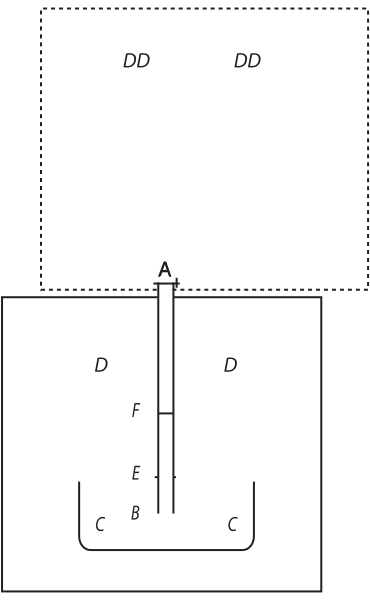
\includegraphics[width=0.4\textwidth]{images/37_3_97v}\\\textit{[Fig. 1]}
%                        %\caption{Bildbeschreibung}
%                        \end{center}
                        %@ @ @ Dies ist eine Abstandszeile - fuer den Fall, dass mehrere figures hintereinander kommen, ohne dass dazwischen laengerer Text steht. Dies kann zu einer Fahlermeldung fuehren. @ @ @ \\
                     \pstart Ad hanc controversiam quae magni in tota natura momenti  est, dirimendam excogitavi \edtext{Experimentum}{\lemma{Experimentum}\Afootnote{ \textbar\ duplex \textit{ gestr.}\ \textbar\ , quod \textit{ L}}}, quod  mihi demonstrandi vim habere \edtext{videtur. Esto Tubus Torricellianus \textit{AB}}{\lemma{videtur}\Afootnote{ \textit{ (1) }\ , ita ut, nunc  auferatur   \textbar\ vel minuatur \textit{ erg.}\ \textbar\  in aere extra Tubum Torricellianum\protect\index{Sachverzeichnis}{Tubus!Torricellianus|textit}  pressio, relicta intus tensione\protect\index{Sachverzeichnis}{tensio|textit}, nunc contra auferatur  vel minuatur tensio\protect\index{Sachverzeichnis}{tensio|textit} in Tubo, relicta pressione extra  Tubum.   \textbar\ Eventaque observentur \textit{ erg.}\ \textbar\ . \textit{ (2) }\ Esto Tubus Torricellianus\protect\index{Sachverzeichnis}{Tubus!Torricellianus|textit} \textit{AB}. Nam si pressione  minuta nulla substituta tensione\protect\index{Sachverzeichnis}{tensio|textit} contraria, relicta. \textit{ (3) }\  Esto Tubus Torricellianus \textit{AB} \textit{ L}}} vas liquoris stagnantis  ei subjectum \textit{C} totum inclusum vasi clauso \edtext{\textit{D} aere pleno.}{\lemma{clauso}\Afootnote{ \textit{ (1) }\ aere pleno \textit{D}  \textit{(a)}\ Aer \textit{(b)}\ Mercurio\protect\index{Sachverzeichnis}{mercurius|textit} delapso ex \textit{A}  in altitudinem ordinariam~ \textbar~\textit{BE} \textit{ erg.}\ \textbar\  introducatur   \textbar\ per vim \textit{ erg.}\ \textbar\  novus aer  in vas \textit{D} ita ut aer in eo incipiat  nonnihil esse compressus, constat altius   \textbar\ solito \textit{ erg.}\ \textbar\  assurgere Mercurium\protect\index{Sachverzeichnis}{mercurius|textit} in Tubo Torricelliano\protect\index{Sachverzeichnis}{Tubus!Torricellianus|textit} verbi gratia in \textit{F}. Haec contra \textit{ (2) }\ aere sed nonnihil compresso pleno, ita ut \textit{ (3) }\ \textit{D} aere pleno. \textit{ L}}} \edtext{Tubus \textit{A} promineat nonnihil ex vase \textit{D} commissuris tamen ubi exit ita munitis, ut aer externus intrare non possit. Et sit in \textit{A} Epistomium\protect\index{Sachverzeichnis}{epistomium} cujus ope Tubus \textit{AB} possit claudi et aperiri.}{\lemma{Tubus \textit{A}}\Afootnote{[...] aperiri. \textit{ erg.} \textit{ L}}} Delabatur Mercurius\protect\index{Sachverzeichnis}{mercurius} ad altitudinem  ordinariam \textit{BE}. Quo facto ex sententia eorum  qui Funiculum\protect\index{Sachverzeichnis}{funiculus} probant, Tensione\protect\index{Sachverzeichnis}{tensio} materiae tenuis\protect\index{Sachverzeichnis}{materia!tenuis}  in spatio \textit{EA} remanentis, nec dilatationem majorem, \edtext{ac proinde nec descensum ulteriorem}{\lemma{}\Afootnote{ac proinde nec descensum ulteriorem \textit{ erg.} \textit{ L}}}  ferentis suspendetur Mercurius\protect\index{Sachverzeichnis}{mercurius} in altitudine \textit{BE}. Aperiatur ergo Epistomium\protect\index{Sachverzeichnis}{epistomium} in \textit{A} dabiturque aeri  libero aditus, ac proinde aer in \textit{AE} tensus esse desinet.  Eventus jam controversiae decisionem dabit, nam si Tensio\protect\index{Sachverzeichnis}{tensio} Mercurium\protect\index{Sachverzeichnis}{mercurius} suspendit, cessante Tensione\protect\index{Sachverzeichnis}{tensio}, Mercurius\protect\index{Sachverzeichnis}{mercurius}  ex \textit{BE} in vas subjectum delabetur. \edtext{Sin suspensus manebit, Funiculus\protect\index{Sachverzeichnis}{funiculus} sustineri non potest.}{\lemma{Sin}\Afootnote{[...] potest. \textit{ erg.} \textit{ L}}} Quod si ais  delabi non posse quia aer subjectus in vase clauso \textit{D} \edtext{delabente Mercurio\protect\index{Sachverzeichnis}{mercurius} ex tubo \textit{BE} in vas \textit{C}}{\lemma{}\Afootnote{delabente Mercurio\protect\index{Sachverzeichnis}{mercurius} ex   \textbar\ tubo \textit{ erg.}\ \textbar\  \textit{BE} in  \textbar\ vas \textit{ erg.}~\textbar~\textit{C} \textit{ erg.} \textit{ L}}}  exitum non reperiat sed comprimi deberet, negas \edtext{vero [98~r\textsuperscript{o}] in aere libero idem eventurum}{\lemma{vero}\Afootnote{ \textit{ (1) }\ gravitatem massae\protect\index{Sachverzeichnis}{gravitas!massae|textit} \textit{ (2) }\ in aere libero idem eventurum \textit{ L}}}
                     \edtext{ecce experimenti commutationem}{\lemma{ecce}\Afootnote{ \textit{ (1) }\ aliud \textit{ (2) }\ levem \textit{ (3) }\ experimenti commutationem \textit{ L}}} quae hoc  quoque effugium praecludat. Scilicet fiat Experimentum Torricellianum\protect\index{Sachverzeichnis}{experimentum!Torricellianum} in aere libero, at Tubus ipse extremitate \textit{A} intret in clausum. Ut prius Experimentum fiebat  in aere \edtext{clauso}{\lemma{aere}\Afootnote{ \textit{ (1) }\ libero \textit{ (2) }\ clauso \textit{ L}}}, Tubus intrabat in liberum. Imaginare  Tibi in eadem fig. vas \textit{D} aliter locari \edtext{in \textit{DD}}{\lemma{}\Afootnote{in \textit{DD} \textit{ erg.} \textit{ L}}} ita ut  Tubum \textit{AB} cum vase subjecto \textit{C} non includat,  sed haec in aere libero relinquantur, nisi quod Tubus \textit{AB} extremitate \textit{A} intret in vas \textit{DD}. Delapso Mercurio\protect\index{Sachverzeichnis}{mercurius} usque ad altitudinem residuam \textit{BE} \edtext{et si placet a materiae tenuis\protect\index{Sachverzeichnis}{materia!tenuis} in \textit{AE} residuae tensione\protect\index{Sachverzeichnis}{tensio} suspenso}{\lemma{}\Afootnote{et [...] suspenso \textit{ erg.} \textit{ L}}} aperiatur Epistomium\protect\index{Sachverzeichnis}{epistomium} prope 
\textit{A} ut Aer \textso{vasis }[\textit{\textso{DD}}]\edtext{}{\Afootnote{\textit{\textso{D}}\textit{\ L \"{a}ndert Hrsg.}}} \edtext{dividat}{\lemma{[\textit{\textso{DD}}]}\Afootnote{ \textit{ (1) }\ intret \textit{ (2) }\ dividat \textit{ L}}}  sese inter vas [\textit{DD}]\edtext{}{\Afootnote{\textit{D}\textit{\ L \"{a}ndert Hrsg.}}} et spatium \textit{AE} et
%\begin{wrapfigure}{l}{0.66\textwidth}                    
%               % \includegraphics[width=0.3\textwidth]{images/37_3_098r}\includegraphics[width=0.3\textwidth]{images/37_3_98v}
%               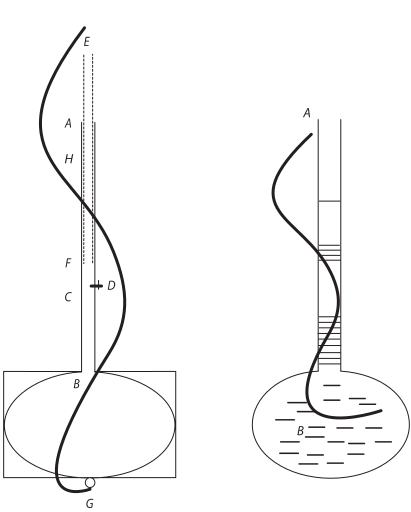
\includegraphics[width=0.6\textwidth]{images/37_3_098ruv}\\\textit{[Fig. 2, ungestr.] \protect\rule[0cm]{2cm}{0cm}\textit{[Fig. 3, gestr.]}}
%                        %\caption{Bildbeschreibung}
%                        \end{wrapfigure} 
                        \edtext{proinde tensio}{\lemma{proinde}\Afootnote{ \textit{ (1) }\ vasis \textit{ (2) }\ tensio \textit{ L}}}  in \textit{AE} diminuetur, tanto magis quanto vas [\textit{DD}]\edtext{}{\Afootnote{\textit{D}\textit{\ L \"{a}ndert Hrsg. } }} est majus. Quia \edtext{enim}{\lemma{enim}\Afootnote{\textbar~tota \textit{ gestr.}~\textbar~tensio \textit{ L}}} 
tensio\protect\index{Sachverzeichnis}{tensio} in \textit{AE} distribuetur  per totum spatium [\textit{DD}]\edtext{}{\Afootnote{D\textit{\ L \"{a}ndert Hrsg. } }} et \textit{AE} simul, non potest non  exigua pars tensionis\protect\index{Sachverzeichnis}{tensio} spatio \textit{AE} obvenire. Quo facto  necesse est, si verus est Funiculus\protect\index{Sachverzeichnis}{funiculus}, seu si Mercurius\protect\index{Sachverzeichnis}{mercurius} Tensione\protect\index{Sachverzeichnis}{tensio}  potius materiae tenuis\protect\index{Sachverzeichnis}{materia!tenuis} tensae in \textit{AE} \edtext{quam contrapondio}{\lemma{quam}\Afootnote{ \textit{ (1) }\ gravitate\protect\index{Sachverzeichnis}{gravitas|textit} \textit{ (2) }\ contrapondio \textit{ L}}} massae\protect\index{Sachverzeichnis}{massa} aereae \edtext{sustinetur; tensione  nunc penitus diminuta, ac}{\lemma{sustinetur;}\Afootnote{ \textit{ (1) }\ cessante nunc tensione\protect\index{Sachverzeichnis}{tensio|textit} ac \textit{ (2) }\ tensione  nunc penitus diminuta, ac \textit{ L}}} pene in nihilum redacta Mercurium\protect\index{Sachverzeichnis}{mercurius} \edtext{\textit{BE}}{\lemma{}\Afootnote{\textit{BE} \textit{ erg.} \textit{ L}}} pene totum delabi in vas \textit{C}  quodsi non fiet, demonstratum est 
%\rule[-4cm]{0cm}{0cm}\clearpage
Funiculum\protect\index{Sachverzeichnis}{funiculus} seu resistentiam materiae\protect\index{Sachverzeichnis}{resistentia!materiae} tenuis (aeris an alterius nihil refert) \edtext{in Tubo relictae}{\lemma{}\Afootnote{in Tubo relictae \textit{ erg.} \textit{ L}}} \edtext{contra}{\lemma{relictae}\Afootnote{ \textit{ (1) }\ ad \textit{ (2) }\ contra \textit{ L}}} \edtext{tensionem\protect\index{Sachverzeichnis}{tensio} suspensi Mercurii causam non esse.\edlabel{98ra}}{\lemma{tensionem}\Afootnote{ \textit{ (1) }\ esse nullam \textit{ (2) }\ suspensi Mercurii causam non esse \textit{ L}}}
%in folio 98v übertragen \edtext{}{\lemma{esse.}
%\Afootnote{ \textit{ (1) }\ Idem ut confirmetur uberius, ac praeterea speciatim  appareat an aer vim patiatur cum tenditur dilataturque  an potius   \textbar\ ipse dilatet sese, id est \textit{ erg.}\ \textbar\  tensio\protect\index{Sachverzeichnis}{tensio|textit} seu dilatatio ipsi sit naturalis, seu an  ipse dilatet sese quantum potest, ubi a nullo circumjecto  premitur; Experimentum hoc instituatur: Esto Ampulla   \textbar\ Follis \textit{ erg.}\ \textbar\  \textit{AB} @@@ G R A F I K @@@ \textit{(a)}\ cujus collum \textit{AC} non \textit{(b)}\ collo oblongo praedita aqua plena praeter partem colli quantamcunque ut \textit{AC} quae  \textit{(aa)}\ Tubi ita exacte \textit{(bb)}\  et antliae\protect\index{Sachverzeichnis}{antlia|textit} vicem praestare possit. Esto paulo supra \textit{C} Epistomium\protect\index{Sachverzeichnis}{epistomium|textit} \textit{D} quo aperto Embolus\protect\index{Sachverzeichnis}{embolus|textit}   \textbar\ \textit{EF} \textit{ erg.}\ \textbar\  collo \textit{AC} exacte  quadrans immittatur in collum \textit{AC}  non tamen usque ad \textit{C} ut relinquatur spatium aere  plenum inter \textit{F} Embolum\protect\index{Sachverzeichnis}{embolus|textit} et \textit{C} aquam, in quod  spatium etiam incidat Epistomium\protect\index{Sachverzeichnis}{epistomium|textit} \textit{D} quod cum sit apertum  aer ab embolo\protect\index{Sachverzeichnis}{embolus|textit} intrante pressus per Epistomium\protect\index{Sachverzeichnis}{epistomium|textit} exibit.  Nunc claudatur Epistomium\protect\index{Sachverzeichnis}{epistomium|textit} Embolusque\protect\index{Sachverzeichnis}{embolus|textit} totis viribus, ex  collo \textit{AF} extrahatur. Et ne follis contrahat sese,  tabulaeque sibi accedant, obstaculo pessulove impediatur.  Sentietur inter extrahendam resistentia ingens.  Claudatur  \textit{(aaa)}\ Tubus \textit{(bbb)}\ \textit{A} ne aer externus intret. Certum  est si foramen   \textbar\ \textit{G} \textit{ erg.}\ \textbar\  aperiatur in Follis \textit{B} tabula quadam,  futurum esse ut aqua subito assurgens repleat  spatium \textit{CD}   \textbar\ Item si foramine \textit{G} clauso manente, obstaculum Tabularum Follis appropinquationem ad se invicem impediens auferatur, follem subito se contracturum, quantum satis sit ut eo in spatium \textit{CH} (aequale spatio \textit{AF}) ascendere aeremque \textit{CF} in maximam amplitudinem seu per totum collum diffusum in priorem dimensionem seu spatium \textit{AH} spatio \textit{CF} aequale, cogere possit. \textit{ erg.}\ \textbar\  Id  \textit{(aaaa)}\ funiculi\protect\index{Sachverzeichnis}{funiculus|textit} patroni fieri dicent,  non \textit{(bbbb)}\  Boylius\protect\index{Namensregister}{\textso{Boyle,} Robert (1627\textendash1691)|textit} aliique fieri dicent,  a pressione Massae aereae\protect\index{Sachverzeichnis}{pressio!aeris|textit} in aquam follis \textit{B} aperti   \textbar\ aut in totum follem clausum \textit{ erg.}\ \textbar\  ab una tantum parte seu a latere \textit{G}  non vero a latere \textit{F} exercitam. Funiculi\protect\index{Sachverzeichnis}{funiculus|textit} defensores  dicent  \textit{(aaaaa)}\ tensionem\protect\index{Sachverzeichnis}{tensio|textit} materiae in \textit{(bbbbb)}\ aerem qui in spatio \textit{FC} residuus manserat ita fuisse tensum, ut coactus  sit replere spatium, totum \textit{AC} hanc autem tensionem\protect\index{Sachverzeichnis}{tensio|textit}  ei esse violentam, eumque conari se contrahere in priores  dimensiones, ac per consequens attrahere aquam  \textit{(aaaaaa)}\ claudere \textit{(bbbbbb)}\  \textit{ (2) }\  \textit{ L}}}
[98 v\textsuperscript{o}] \edtext{Decidi quidem potest\edlabel{98rb}}{\lemma{esse.}\xxref{98ra}{98rb}\Afootnote{\textit{ (1) }\ Idem ut confirmetur uberius, ac praeterea speciatim  appareat an aer vim patiatur cum tenditur dilataturque  an potius   \textbar\ ipse dilatet sese, id est \textit{ erg.}\ \textbar\  tensio\protect\index{Sachverzeichnis}{tensio|textit} seu dilatatio ipsi sit naturalis, seu an  ipse dilatet sese quantum potest, ubi a nullo circumjecto  premitur; Experimentum hoc instituatur: Esto Ampulla   \textbar\ Follis \textit{ erg.}\ \textbar\  \textit{AB} \textit{(a)}\ cujus collum \textit{AC} non \textit{(b)}\ collo oblongo praedita aqua plena praeter partem colli quantamcunque ut \textit{AC} quae  \textit{(aa)}\ Tubi ita exacte \textit{(bb)}\  et antliae\protect\index{Sachverzeichnis}{antlia|textit} vicem praestare possit. Esto paulo supra \textit{C} Epistomium\protect\index{Sachverzeichnis}{epistomium|textit} \textit{D} quo aperto Embolus\protect\index{Sachverzeichnis}{embolus|textit}   \textbar\ \textit{EF} \textit{ erg.}\ \textbar\  collo \textit{AC} exacte  quadrans immittatur in collum \textit{AC}  non tamen usque ad \textit{C} ut relinquatur spatium aere  plenum inter \textit{F} Embolum\protect\index{Sachverzeichnis}{embolus|textit} et \textit{C} aquam, in quod  spatium etiam incidat Epistomium\protect\index{Sachverzeichnis}{epistomium|textit} \textit{D} quod cum sit apertum  aer ab embolo\protect\index{Sachverzeichnis}{embolus|textit} intrante pressus per Epistomium\protect\index{Sachverzeichnis}{epistomium|textit} exibit.  Nunc claudatur Epistomium\protect\index{Sachverzeichnis}{epistomium|textit} Embolusque\protect\index{Sachverzeichnis}{embolus|textit} totis viribus, ex  collo \textit{AF} extrahatur. Et ne follis contrahat sese,  tabulaeque sibi accedant, obstaculo pessulove impediatur.  Sentietur inter extrahendam resistentia ingens.  Claudatur  \textit{(aaa)}\ Tubus \textit{(bbb)}\ \textit{A} ne aer externus intret. Certum  est si foramen~\textbar~\textit{G} \textit{ erg.}~\textbar~aperiatur in Follis \textit{B} tabula quadam,  futurum esse ut aqua subito assurgens repleat  spatium \textit{CD}~\textbar~Item si foramine \textit{G} clauso manente, obstaculum Tabularum Follis appropinquationem ad se invicem impediens auferatur, follem subito se contracturum, quantum satis sit ut eo in spatium \textit{CH} (aequale spatio \textit{AF}) ascendere aeremque \textit{CF} in maximam amplitudinem seu per totum collum diffusum in priorem dimensionem seu spatium \textit{AH} spatio \textit{CF} aequale, cogere possit. \textit{ erg.}\ \textbar\  Id  \textit{(aaaa)}\ funiculi\protect\index{Sachverzeichnis}{funiculus|textit} patroni fieri dicent,  non \textit{(bbbb)}\  Boylius\protect\index{Namensregister}{\textso{Boyle} (Boylius, Boyl., Boyl), Robert 1627\textendash 1691|textit} aliique fieri dicent,  a pressione Massae aereae\protect\index{Sachverzeichnis}{pressio!aeris|textit} in aquam follis \textit{B} aperti   \textbar\ aut in totum follem clausum \textit{ erg.}\ \textbar\  ab una tantum parte seu a latere \textit{G}  non vero a latere \textit{F} exercitam. Funiculi\protect\index{Sachverzeichnis}{funiculus|textit} defensores  dicent  \textit{(aaaaa)}\ tensionem\protect\index{Sachverzeichnis}{tensio|textit} materiae in \textit{(bbbbb)}\ aerem qui in spatio \textit{FC} residuus manserat ita fuisse tensum, ut coactus  sit replere spatium, totum \textit{AC} hanc autem tensionem\protect\index{Sachverzeichnis}{tensio|textit}  ei esse violentam, eumque conari se contrahere in priores  dimensiones, ac per consequens attrahere aquam  \textit{(aaaaa-a)}\ claudere \textit{(bbbbb-b)}\  ex Folle \textit{B} ubi potuerit. Non potuisse autem  donec follis claudi aut aer in eum intrare  potuerit. Controversia ita dirimetur. Manente \textit{A} et \textit{G} et \textit{D} clausis, et  obstaculo Tabularum follis approximationem  impediente non ablato \textit{ (2) }\   Idem, an aer \hspace{2mm}scilicet tendenti \textbar\ seu dilatanti \textit{ erg.}\ \textbar\  resistat, alio Experimento  ita explorari potest: Esto  \textit{ (3) }\   Demonstratum quidem est \textit{ (4) }\ Decidi quidem potest \textit{ L}}} hoc experimento, et quod  sciam hactenus unico (caetera enim \edtext{fere}{\lemma{enim}\Afootnote{ \textit{ (1) }\ pene omnia \textit{ (2) }\ fere \textit{ L}}} \edtext{aeque}{\lemma{}\Afootnote{aeque \textit{ erg.} \textit{ L}}} per funiculum\protect\index{Sachverzeichnis}{funiculus} \edtext{ac per aeris gravitatem\protect\index{Sachverzeichnis}{gravitas!aeris}}{\lemma{}\Afootnote{ac per aeris gravitatem\protect\index{Sachverzeichnis}{gravitas!aeris} \textit{ erg.} \textit{ L}}} explicari potuere) \edtext{an aeris tensio an vero gravitas sit causa proxima}{\lemma{potuere)}\Afootnote{ \textit{ (1) }\ Aeris tensionem\protect\index{Sachverzeichnis}{tensio|textit}  non esse causam \textit{ (2) }\ an [...] proxima \textit{ L}}} Mercurii\protect\index{Sachverzeichnis}{mercurius} suspensi; 
 %\begin{wrapfigure}{l}{0.2\textwidth}                    
     %           \includegraphics[width=0.2\textwidth]{images/37_3_98v}\\\textit{[Fig. 2, gestr.]}
                        %\caption{Bildbeschreibung}
         %               \end{wrapfigure}
                        %@ @ @ Dies ist eine Abstandszeile - fuer den Fall, dass mehrere figures hintereinander kommen, ohne dass dazwischen laengerer Text steht. Dies kann zu einer Fahlermeldung fuehren. @ @ @ \\
                   %  \edtext{}{\lemma{suspensi;}\Bfootnote{Zeichnung gestrichen}} 
                   at vero  non potest decidi altera quae remanet quaestio, Aerne \edtext{suapte}{\lemma{Aerne}\Afootnote{ \textit{ (1) }\ sit  \textit{ (2) }\ suapte \textit{ L}}} natura \edtext{dilatetur}{\lemma{natura}\Afootnote{ \textit{ (1) }\ tendi possi \textit{ (2) }\ dilatetur \textit{ L}}}, ubi scilicet  pressio ambientis \edtext{cessat,}{\lemma{cessat,}\Afootnote{\textbar\ ut sentire videtur Boylius\protect\index{Namensregister}{\textso{Boyle} (Boylius, Boyl., Boyl), Robert 1627\textendash 1691}, \textit{ gestr.}\ \textbar\ an \textit{ L}}}  an vero potius ambiente abstracto ad locum implendum  per vim distendatur? Ac proinde an  aer summus sit magis tensus inferiore, an saltem  minus pressus. Sed ne accurate expensa videtur haec quaestio  ei similis esse, \edtext{quam movent, an}{\lemma{esse,}\Afootnote{ \textit{ (1) }\ an scilicet \textit{ (2) }\ quam movent, an \textit{ L}}} satius sit \edtext{supponere}{\lemma{sit}\Afootnote{ \textit{ (1) }\ imaginari simi \textit{ (2) }\ supponere \textit{ L}}} omnia \edtext{Elementa\protect\index{Sachverzeichnis}{elementum} gravia}{\lemma{Elementa}\Afootnote{ \textit{ (1) }\ levia \textit{ (2) }\  gravia \textit{ L}}}, et minus grave per consequens in summo,  an cum docto quodam nostri temporis philosopho \edtext{credere}{\lemma{philosopho}\Afootnote{ \textit{ (1) }\ supponere \textit{ (2) }\ credere \textit{ L}}} omnia \edtext{esse}{\lemma{}\Afootnote{esse \textit{ erg.} \textit{ L}}} levia, \edtext{et a centro per circulationem terrae\protect\index{Sachverzeichnis}{circulatio!terrae} rejecta}{\lemma{}\Afootnote{et [...] rejecta \textit{ erg.} \textit{ L}}}, et minus leve in fundo. Revera  enim nec gravia nec levia sunt \edtext{corpora}{\lemma{}\Afootnote{corpora \textit{ erg.} \textit{ L}}} nisi per \edtext{comparationem.}{\lemma{comparationem.}\Bfootnote{\textsc{R. Descartes, }\cite{00035}\textit{Principia philosophiae}, Amsterdam 1644, S.~200 (\textit{DO} VIII, 1, S.~213).}}  Eodem modo ajo nec tensionem\protect\index{Sachverzeichnis}{tensio} nec compressionem\protect\index{Sachverzeichnis}{compressio} corporibus ipsis  esse violentam. \edtext{Nam si}{\lemma{violentam.}\Afootnote{ \textit{ (1) }\ Sed p \textit{ (2) }\ Nam si \textit{ L}}} dicis compressionem\protect\index{Sachverzeichnis}{compressio} esse  violentam, \edtext{cur non potius}{\lemma{violentam,}\Afootnote{ \textit{ (1) }\ nulla est \textit{ (2) }\ cur non potius \textit{ L}}} tensionem\protect\index{Sachverzeichnis}{tensio}, \edtext{si tensionem\protect\index{Sachverzeichnis}{tensio}, cur non potius compressionem\protect\index{Sachverzeichnis}{compressio},}{\lemma{}\Afootnote{si [...] compressionem\protect\index{Sachverzeichnis}{compressio}, \textit{ erg.} \textit{ L}}} semper  enim quantum tenditur hic tantum alibi comprimitur.  Vis ergo tendendo comprimendoque, elevando et deprimendo  non singulis corporibus, sed \edtext{toti affertur}{\lemma{sed}\Afootnote{ \textit{ (1) }\ Universo\protect\index{Sachverzeichnis}{universum|textit} affertur \textit{ (2) }\ toti affertur \textit{ L}}}. \edtext{Quia circulatio universalis  quam Lux}{\lemma{affertur.}\Afootnote{ \textit{ (1) }\ Totius enim massae\protect\index{Sachverzeichnis}{massa|textit} circulatio \textit{ (2) }\  Circulatio enim Lucis \textit{ (3) }\ Quia circulatio universalis  quam Lux \textit{ L}}} circa globum nostrum exercet, \edtext{corpora compressa, id est}{\lemma{exercet,}\Afootnote{ \textit{ (1) }\ corpora  \textit{(a)}\ alibi \textit{(b)}\ colligit comprimitque, alibi \textit{ (2) }\ prope \textit{ (3) }\ majorem massae\protect\index{Sachverzeichnis}{massa|textit}  partem \textit{ (4) }\ corpora compressa, id est \textit{ L}}} motu proprio fortiore praedita,  (experimentis enim demonstrari potest\edtext{}{\lemma{}\Afootnote{potest  \textbar\ omnia \textit{ gestr.}\ \textbar\ compressa \textit{ L}}} compressa  habere motum intestinum fortem, dilatata seu tensa  languidum \edtext{de quo suo loco fusius dicam, et rem veteribus inter certa, philosophis recentioribus inter vana Scholasticorum figmenta habitam demonstrabo, idem corpus sine ulla materia subtili intrante aut expressa modo majorem modo minorem locum implere posse}{\lemma{}\Afootnote{de [...] certa, \textit{ (1) }\ nostris philosophis \textit{ (2) }\ philosophis [...] corpus \textit{(a)}\ modo plus modo minus spatii \textit{(b)}\ sine [...] expressa \textit{(aa)}\ eundem locum \textit{(bb)}\ modo majorem modo minorem locum implere posse \textit{ erg.} \textit{ L}}}) ac proinde motum universalem\protect\index{Sachverzeichnis}{motus!universalis} magis  turbantia cogit ad locum ubi motus universalis\protect\index{Sachverzeichnis}{motus!universalis} facilius  turbari potest, seu languidior est, id est versus centrum.  Et dilatatiora proinde a centro \edtext{\edlabel{repi1}repellit.}{\lemma{repellit.}\Afootnote{ \textit{ erg.} \textit{ L}}} \edtext{Quod}{\lemma{repellit.}\xxref{repi1}{repi2}\Afootnote{ \textit{ (1) }\ Et in loco  a centro aeque distante repugna \textit{ (2) }\ Resistit \textit{ (3) }\ Et \textit{ (4) }\ aut \textit{ (5) }\  Quod \textit{ L}}} si \edtext{\edlabel{repi2}dilatatiora a centro,}{\lemma{si}\Afootnote{ \textit{ (1) }\ ea a centro repell \textit{ (2) }\ dilatatiora   \textbar\ a centro \textit{ erg.}\ \textbar\ , \textit{ L}}} aut  compressiora ad centrum ob obstacula movere negat;  disjiciet compressa, comprimet dilatata, prout locus  id est corporum circumjacentium status requiret.  Pendent ergo phaenomena illa omnia a conatu Naturae\protect\index{Sachverzeichnis}{conatus!naturae} universali ad uniformitatem, \edtext{seu}{\lemma{uniformitatem,}\Afootnote{ \textit{ (1) }\ id est in loc \textit{ (2) }\ seu \textit{ L}}} ubi  eadem ratio est, ad aequalitatem; ubi diversa, ad proportionem.  Experimenta ergo omnia quae vulgo Fugae Vacui\protect\index{Sachverzeichnis}{fuga vacui} tribuuntur, \edtext{et a doctissimis philosophis nostro tempore ponderi aeris  ascripta sunt}{\lemma{tribuuntur,}\Afootnote{ \textit{ (1) }\ asseruntur \textit{ (2) }\ et [...] sunt \textit{ L}}} 
                     habent \edtext{causam universalem:}
                     {\lemma{causam}\Afootnote{\textbar\ propriam \textit{ gestr.}\ \textbar\ universalem: \textit{ L}}}  
                     %Sperrung auskommentiert
                    %\textso{}\protect\index{Sachverzeichnis}{conatus!naturae}  
                   \textso{conatum Naturae ad uniformitatem}
                     %Sperrung Ende
                     cujus exemplum tantum caeteris  frequentius, in Aeris Gravitate\protect\index{Sachverzeichnis}{gravitas!aeris} atque Elaterio\protect\index{Sachverzeichnis}{elaterium} esse, ac proinde  phaenomena illa saepe quidem, non semper tamen his deberi ex sequentibus  Experimentis partim jam publicatis, partim nunc a me propositis patebit.   \pend 